% !TEX TS-program = xelatex
% !BIB TS-program = bibtex
\documentclass[12pt,letterpaper]{article}
\usepackage{style/dsc180reportstyle} % import dsc180reportstyle.sty
\usepackage{float} % for [H] figure placement

%%%%%%%%%%%%%%%%%%%%%%%%%%%%%%%%%%%%%%%%%%%%%%%%%%%%%%%%
%%%% Title and Authors
%%%%%%%%%%%%%%%%%%%%%%%%%%%%%%%%%%%%%%%%%%%%%%%%%%%%%%%%

\title{DSC Capstone Q1 Report}

\author{Jevan Chahal\\
  {\tt j2chahal@ucsd.edu} \\\And
  Hillary Change \\
  {\tt hic001@ucsd.edu} \\\And
  Kurumi Kaneko \\
  {\tt kskaneko@ucsd.edu} \\\And
  Kevin Wong \\
  {\tt kew024@ucsd.edu} \\\And
  Brian Duke \\
  {\tt brian.duke@prismdata.com} \\\And
  Kyle Nero \\
  {\tt kyle.nero@prismdata.com} \\}

\begin{document}
\maketitle

%%%%%%%%%%%%%%%%%%%%%%%%%%%%%%%%%%%%%%%%%%%%%%%%%%%%%%%%
%%%% Abstract and Links
%%%%%%%%%%%%%%%%%%%%%%%%%%%%%%%%%%%%%%%%%%%%%%%%%%%%%%%%

\begin{abstract}
    \textcolor{Black}{
    The process of capturing what makes a creditor trustworthy or not is especially vital within the confines of bank data, due to the guidelines and ethics of what makes this data usable. Although the quantity of the data is massive, there are only a few available features that are explicitly useful in the confines of machine learning, which calls into question how we should measure customer's trustworthiness towards their creditors. Our methodology details the process of refining bank data into categories using Natural Language Processing, assessing individual's income based on bank data alone, and also measuring their credit worthiness both accurately and efficiently. 
    }
\end{abstract}

\begin{center}
Code: \url{https://github.com/hillarychang/dsc180a-capstone-q1}
\end{center}

\maketoc
\clearpage

%%%%%%%%%%%%%%%%%%%%%%%%%%%%%%%%%%%%%%%%%%%%%%%%%%%%%%%%
%%%% Main Contents
%%%%%%%%%%%%%%%%%%%%%%%%%%%%%%%%%%%%%%%%%%%%%%%%%%%%%%%%

\section{Introduction}
Predicting a customer’s creditworthiness is an essential task for banks, as it informs decisions relating to the profitability and risks of loans, credit cards, and other financial services. While traditional credit scores are widely used, they often overlook important aspects of customer behavior, especially for individuals with limited credit history. We aim to develop an alternative approach by analyzing transaction data to create a new creditworthiness measure, which we will call the "Blank Score." By examining patterns in spending, income consistency, and transaction types, we hope to create a model that more accurately reflects individual financial reliability.

\subsection{Data Description}
The dataset, provided by Prism Data, consists of detailed transaction records that include fields such as \texttt{memo}, \texttt{amount}, \texttt{date}, and \texttt{category}.
\begin{itemize}
    \item \textbf{\texttt{prism\_consumer\_id} (Quantitative):} Unique identifier for each consumer, used to analyze spending and income patterns per user.
    \item \textbf{\texttt{prism\_account\_id} (Qualitative):} Identifier for each account, distinguishing multiple accounts for a single consumer or across consumers.
    \item \textbf{\texttt{memo} (Qualitative):} Descriptive text providing transaction details, such as "grocery store" or "ATM withdrawal," useful for categorization.
    \item \textbf{\texttt{amount} (Quantitative):} Transaction value, where positive values represent inflows (e.g., deposits) and negative values represent outflows (e.g., payments).
    \item \textbf{\texttt{posted\_date} (Qualitative):} Date each transaction was posted, enabling temporal analysis of spending trends.
    \item \textbf{\texttt{category} (Qualitative):} Pre-assigned transaction type label, such as "food" or "utilities," serving as a basis for categorization.
\end{itemize}

\subsection{Exploratory Data Analysis}
We first conducted Exploratory Data Analysis using transaction data given to us from our industry partner, Prism Data. This analysis allowed us to identify different patterns. In specific, we observed notable differences in spending behaviors across various time periods. For instance, we noticed that most purchases occurred on weekdays, while weekends had significantly less purchasing priority, suggesting that consumers prioritize certain purchases during the week. 

We also examined seasonal patterns within the dataset, which spans from 2020 to 2023. Certain months, like April and May, showed increased inflows likely due to tax returns, while December exhibited higher spending, likely due to holiday-related expenses. These patterns indicate regular income and expenditure behaviors that could be relevant for predicting creditworthiness.

\begin{figure}[H]
    \centering
    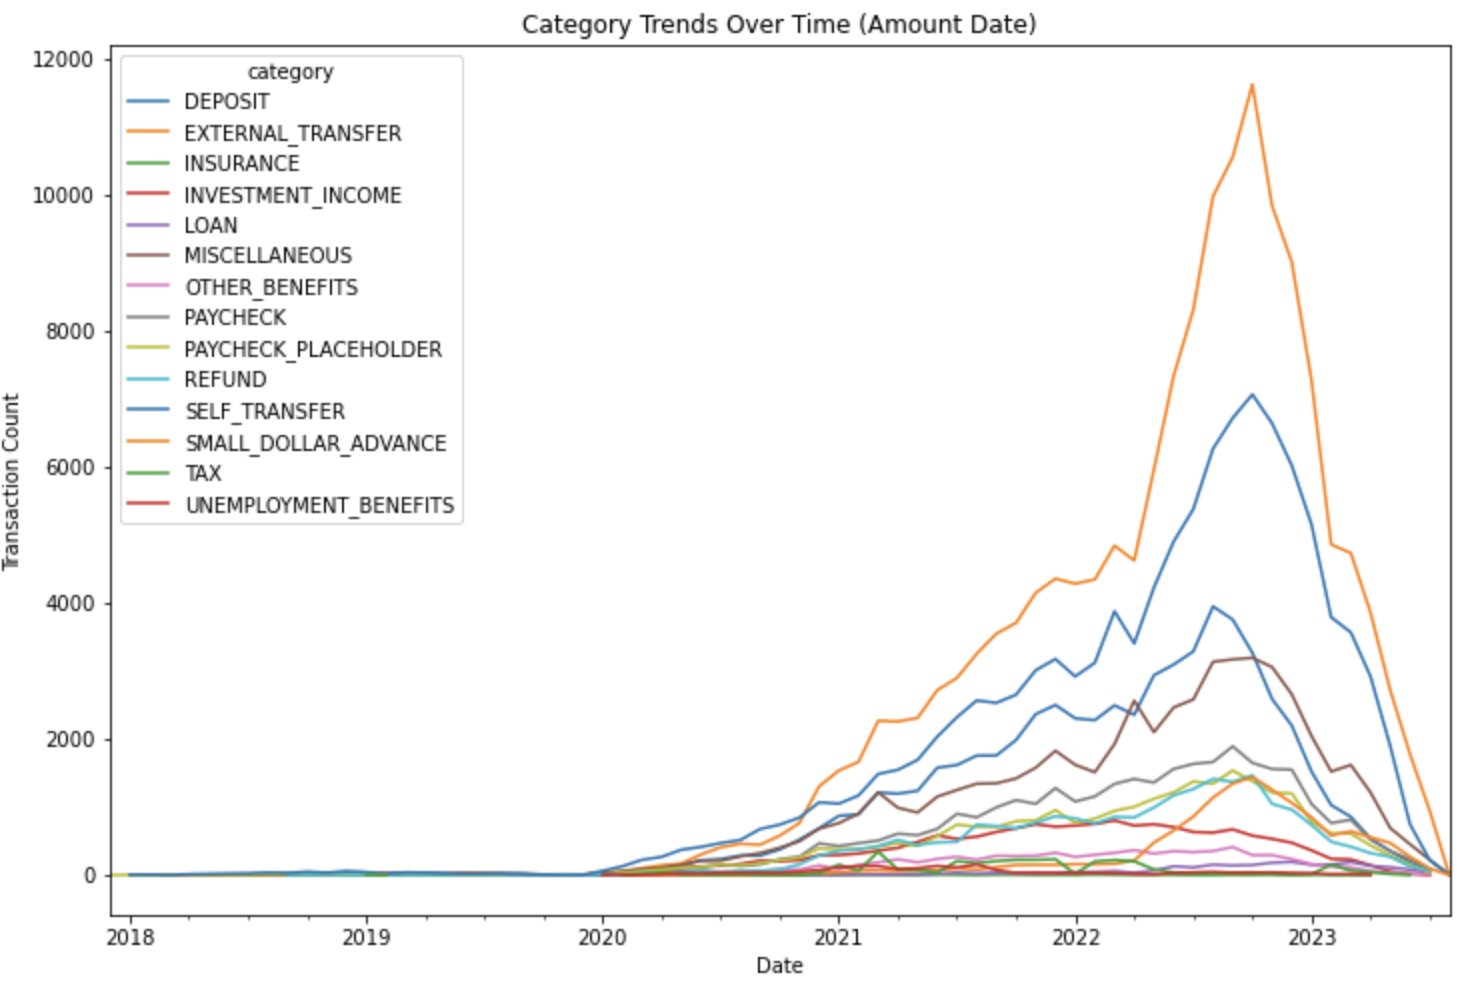
\includegraphics[width=\textwidth]{figure/category_time.png}
    \caption{Trends of transaction categories over time. This exploratory analysis visualizes patterns in transaction volume across different categories, showing insights such as seasonal spending behavior and category-specific peaks. For example, categories like \texttt{DEPOSIT} and \texttt{EXTERNAL\_TRANSFER} show higher transaction counts in certain months.}
    \label{fig:category_trends}
\end{figure}

\begin{figure}[H]
    \centering
    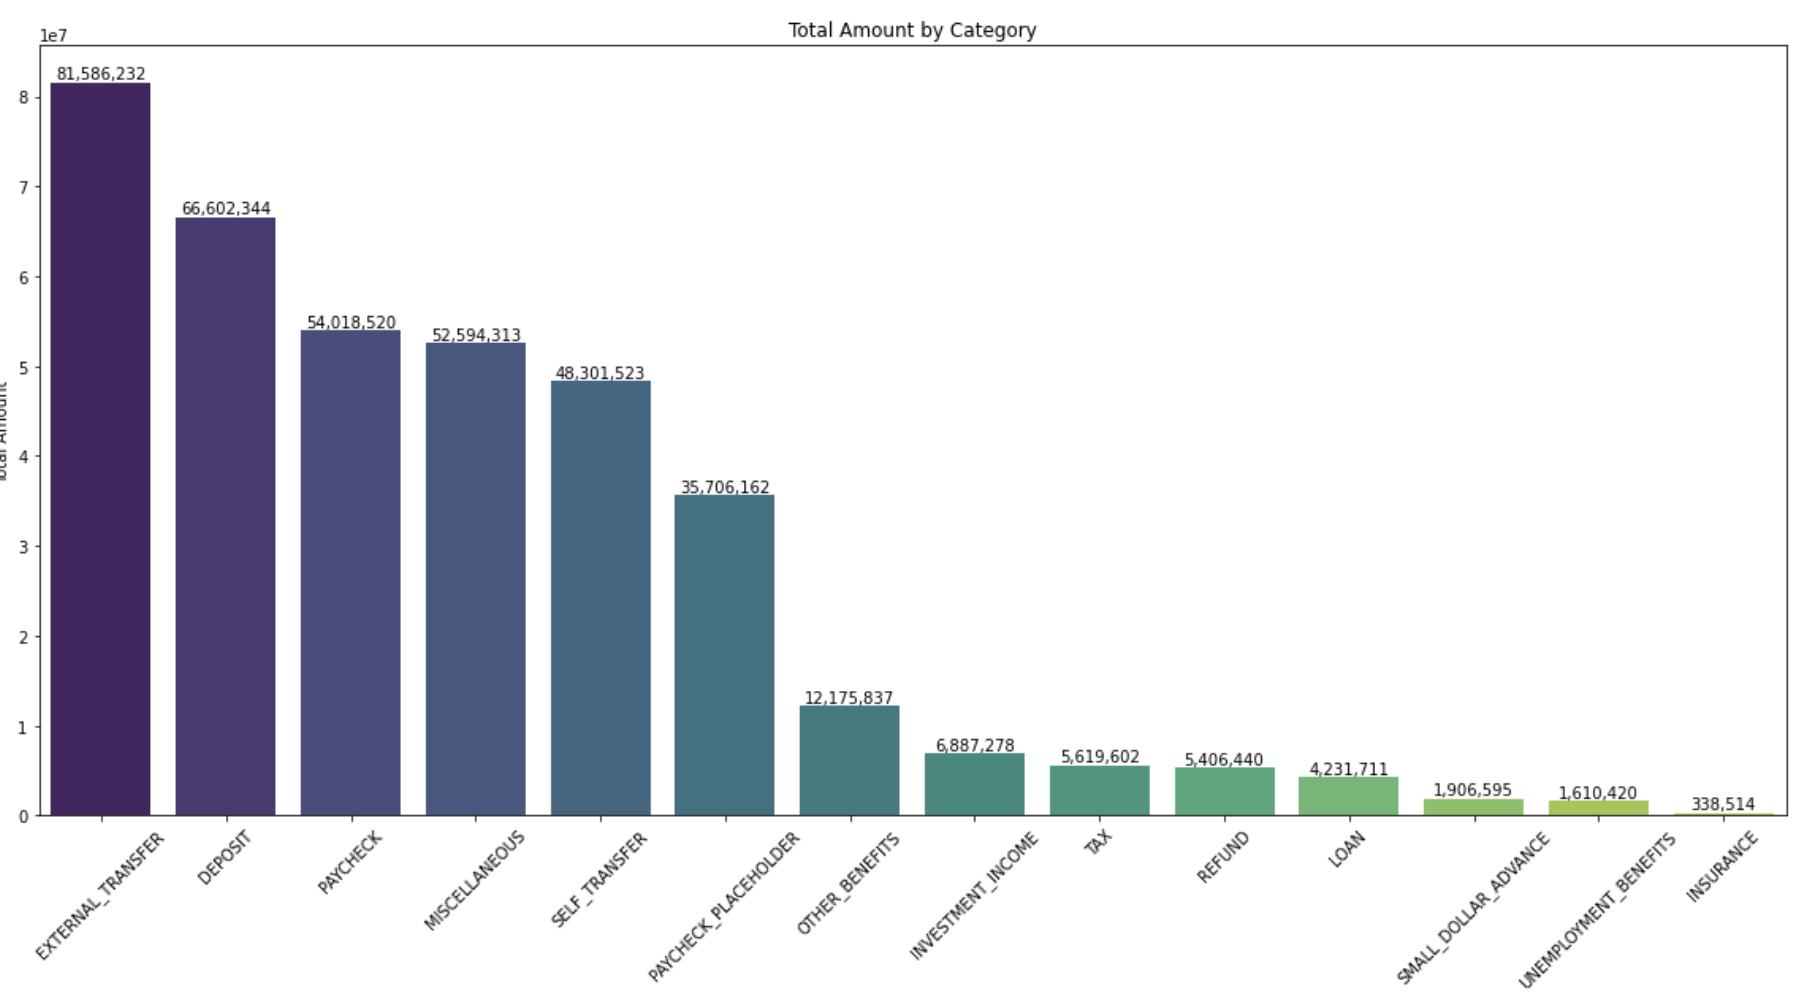
\includegraphics[width=\textwidth]{figure/amt_category.png}
    \caption{Bar chart showing the total amount spent across categories. This visualization highlights which categories contribute the most to overall expenditure, with \texttt{EXTERNAL\_TRANSFER}, \texttt{DEPOSIT}, and \texttt{PAYCHECK} as leading contributors. This information is valuable for understanding the primary financial activities within the dataset.}
    \label{fig:total_amount_by_category}
\end{figure}

\subsection{Train-Test Split and Data Distribution}
\begin{figure}[H]
    \centering
    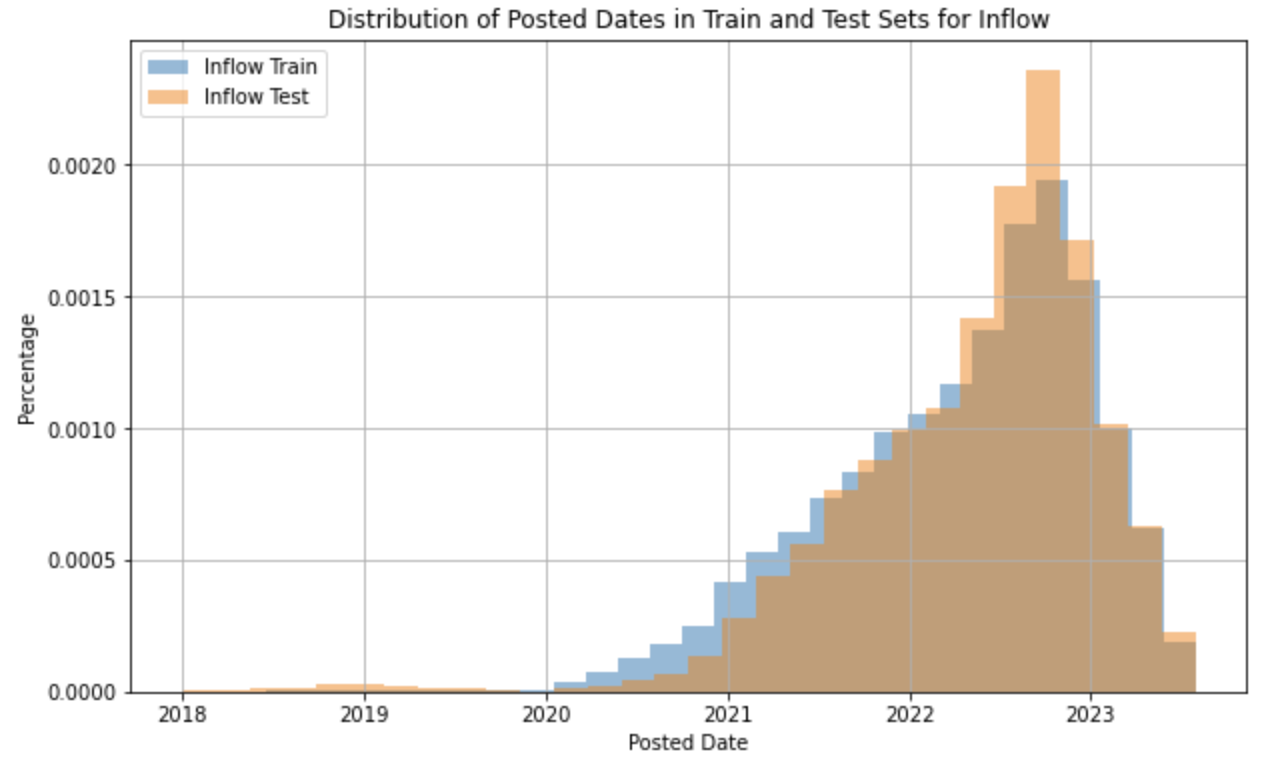
\includegraphics[width=\textwidth]{figure/inflow.png}
    \caption{Histogram of posted dates for the Inflow dataset. The distribution between training and testing sets is almost identical, indicating that the split was performed evenly across time periods. This ensures that both sets are representative of the overall data distribution and reduces potential biases when developing models.}
    \label{fig:inflow_date_distribution}
\end{figure}

\begin{figure}[H]
    \centering
    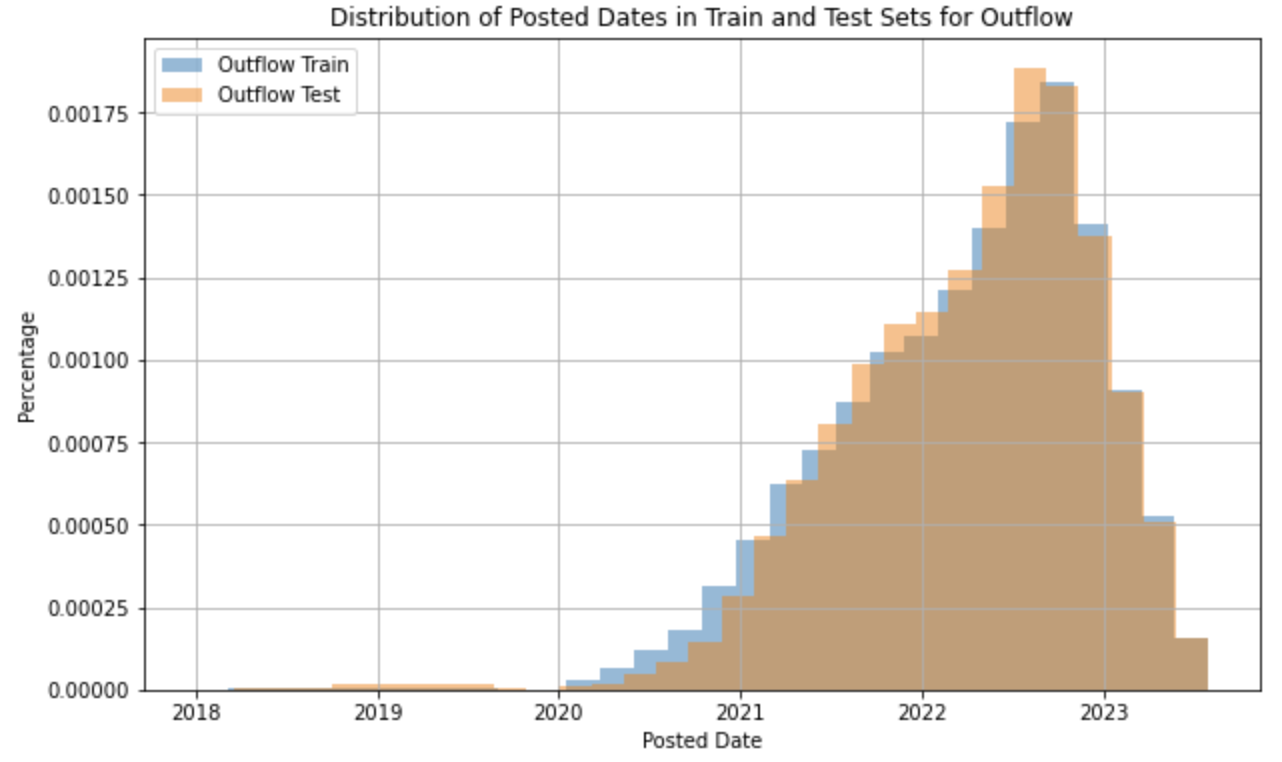
\includegraphics[width=\textwidth]{figure/outflow.png}
    \caption{Histogram of posted dates for the Outflow dataset. Similar to the Inflow dataset, the distribution of dates is balanced between the training and testing sets, verifying an even temporal split. This helps in maintaining consistency and prevents temporal biases in model training and evaluation.}
    \label{fig:outflow_date_distribution}
\end{figure}

\section{Methods}
\subsection{Data Cleaning}
To prepare the memo field for analysis, we first applied a series of cleaning steps to standardize the text. We transformed all text to lowercase for uniformity, removed any extraneous punctuation and symbols, and stripped out dates, state abbreviations, and recurring text that didn’t contribute to transaction categorization (ex., “POS withdrawal”). We also removed placeholder values, such as multiple X’s.

To prepare the dataset for modeling, we began by reviewing a sample of unique transaction memos from each category. This step provided insights into common patterns and inconsistencies, helping us determine the scope and focus of our cleaning tasks.

\begin{figure}[H]
    \centering
    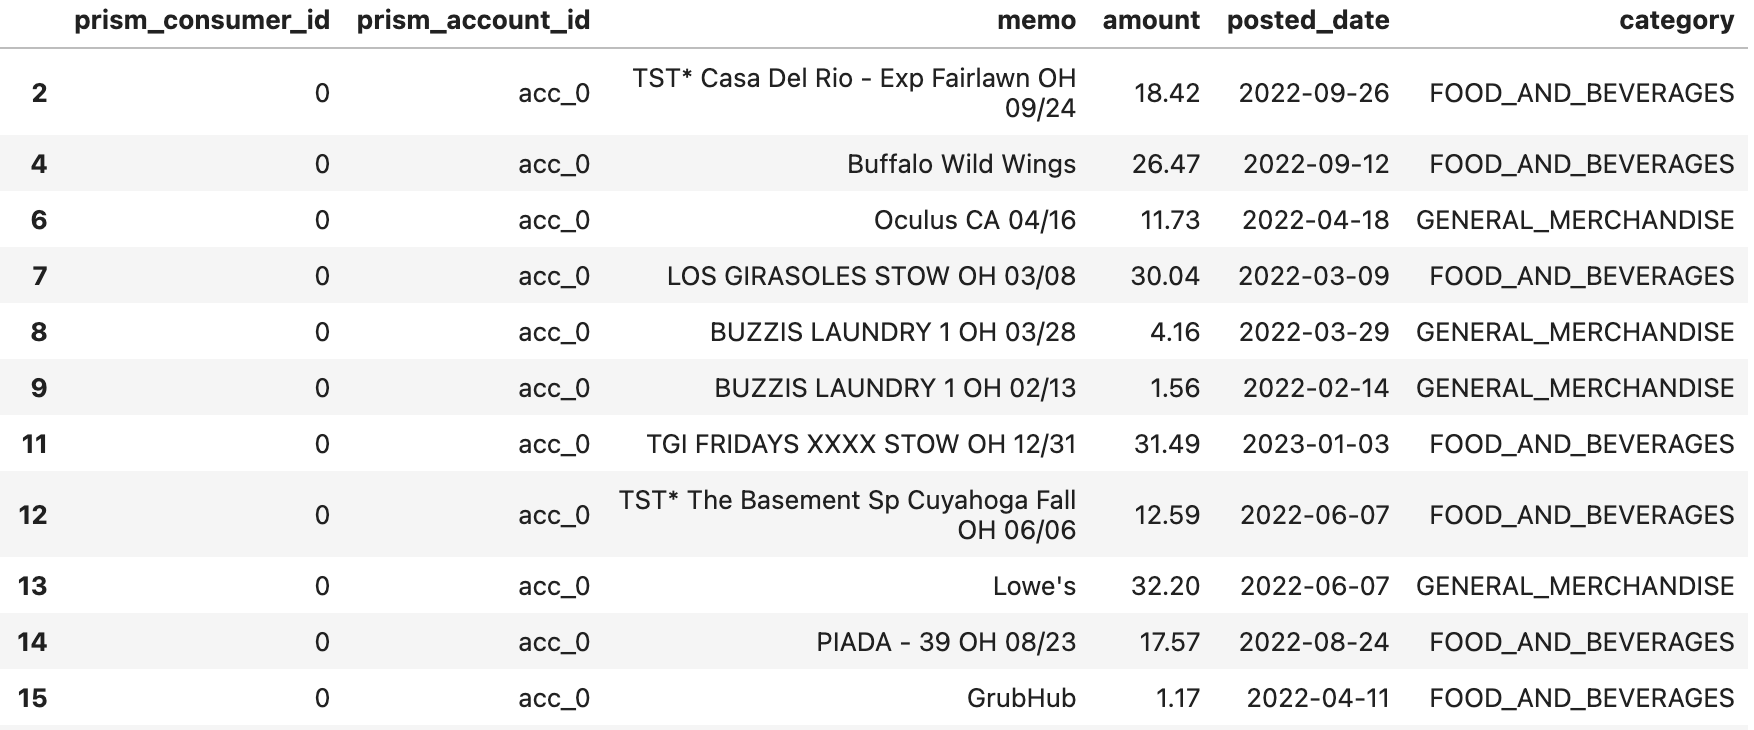
\includegraphics[width=\textwidth]{figure/nonclean_df.png}
    \caption{This table shows the memo dataframe before cleaning. Variations in text format, inconsistent capitalization, and extraneous characters can be observed, which motivated the cleaning process to improve uniformity in transaction descriptions.}
    \label{fig:pre_cleaned_memo}
\end{figure}

We then applied several transformations to standardize the data and improve its interpretability:

\begin{enumerate}
    \item \textbf{Date Removal}: We used regular expressions (RegEx) to locate and remove dates across entries in the memo column, as they did not contribute to the model's predictive goals and added unnecessary complexity. We also removed any extraneous or ambiguous patterns (e.g., “XXXX” entries).

    \item \textbf{Pattern Recognition}: Specific patterns and keywords were identified as indicators of certain transaction categories. For example, "TST" reliably associated with "Food and Beverages," while strings like "APPLE.COM/BILL" were linked to "General Merchandise." We flagged these patterns to automate future classifications and reduce manual intervention.

    \item \textbf{Selective Character Retention}: To preserve potentially valuable information, we retained certain characters such as dots ('.'). This choice allowed us to keep URLs or email addresses within the memo field, which could provide clues to the transaction category.

    \item \textbf{Transaction Labels}: We also identified recurring phrases such as "POS Withdrawal," location-specific markers (e.g., “CA 10/27” for state and date), and labels indicating recurring payments. These were removed for as they did not contribute to the model's predictive goals and added unnecessary complexity.

    \item \textbf{Text Normalization}: All text was converted to lowercase to reduce variability due to case differences.
\end{enumerate}

By implementing these steps, we improved data consistency and ensured key transactional information was preserved, enhancing our model's ability to accurately predict customer creditworthiness.

\begin{figure}[H]
    \centering
    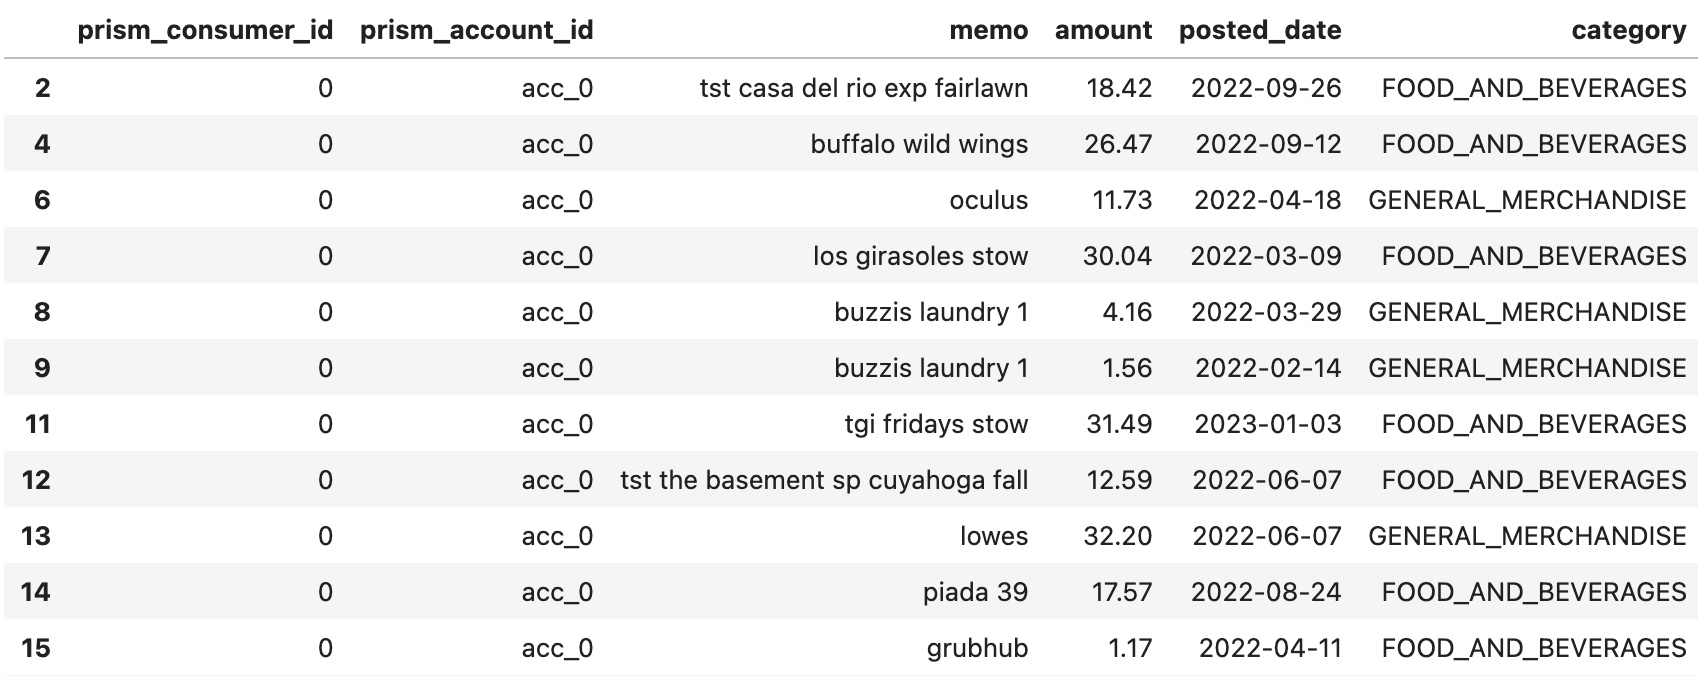
\includegraphics[width=\textwidth]{figure/clean_df.jpeg}
    \caption{This table represents the cleaned memo dataframe, where we applied text preprocessing to ensure consistency across transaction descriptions. By converting to lowercase, removing punctuation, and standardizing certain tokens, we prepared the data for more accurate feature extraction and analysis.}
    \label{fig:clean_memo}
\end{figure}

\subsection{Token Augmentation}
To prepare the transaction data for further analysis and modeling, we enhanced the `memo` field by adding specific tokens based on transaction characteristics. This token augmentation adds additional context about transaction amounts and dates, helping the model learn more meaningful patterns. 

\begin{figure}[h]
    \centering
    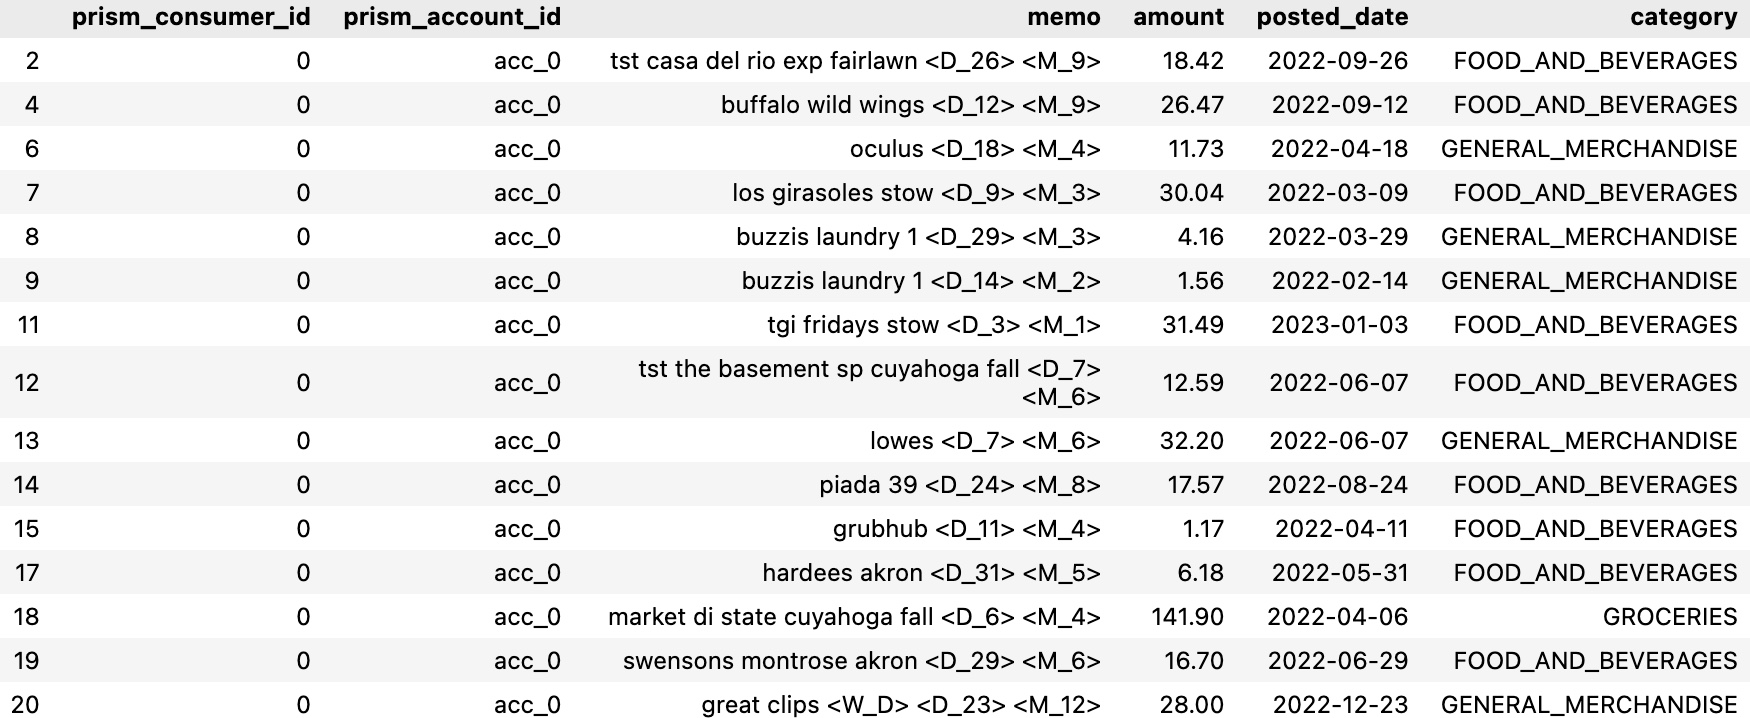
\includegraphics[width=\textwidth]{figure/pre_token.jpeg}
    \caption{This is the transaction data cleaned but not token augmented yet. The \texttt{memo} field contains raw text descriptions without any added tokens.}
    \label{fig:cleaned_data}
\end{figure}

The following steps outline the transformation process:

\begin{enumerate}
    \item \textbf{Whole Dollar Amount Identification}: We added a token \texttt{<W\_D>} to the `memo` field for transactions with whole dollar amounts. This token is useful for identifying transactions that might involve cash withdrawals or ATM transactions, as these are typically in round dollar amounts (e.g., \$20, \$50) since people rarely withdraw amounts with cents.

    \item \textbf{Day of Transaction}: For each transaction's posting date, we generated a day token in the format \texttt{<D\_day>}, where \texttt{day} represents the specific day of the month. This token provides temporal information, which could be helpful for analyzing patterns such as end-of-month or beginning-of-month spending habits.

    \item \textbf{Month of Transaction}: Similarly, we generated a month token in the format \texttt{<M\_month>} (where \texttt{month} is the numerical month) to capture any potential seasonal or monthly trends in spending behavior.

    \item \textbf{Token Augmentation Process}: For each row in the token augmented outflows DataFrame, we concatenated these tokens to the `memo` field:

    \begin{verbatim}
    memo = memo + whole_dollar_amount_token + day_token + month_token
    \end{verbatim}

    where \texttt{whole\_dollar\_amount\_token}, \texttt{day\_token}, and \texttt{month\_token} represent the applicable tokens based on each transaction's attributes.

\end{enumerate}

\begin{figure}[h]
    \centering
    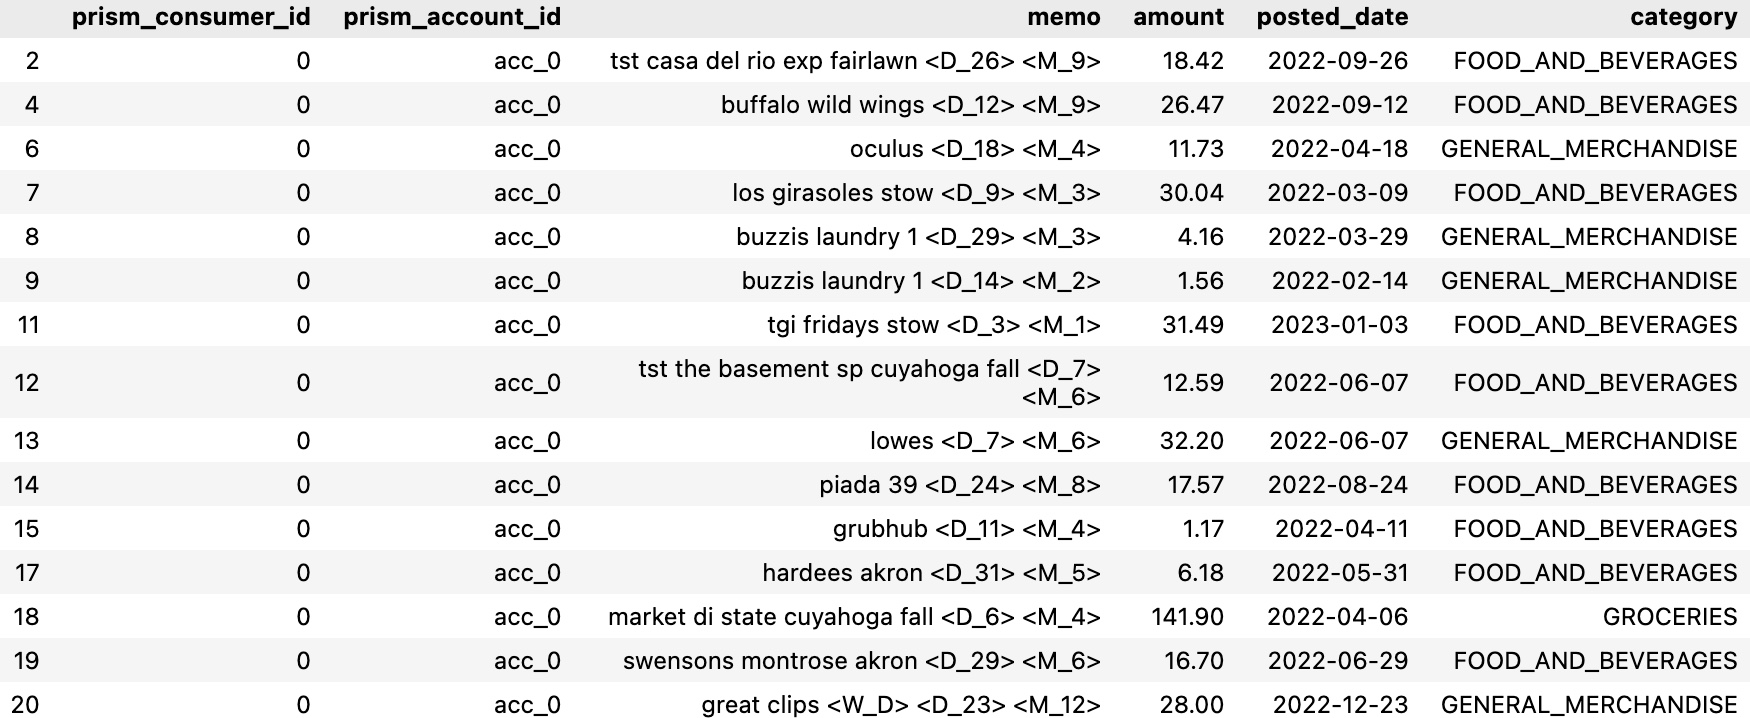
\includegraphics[width=\textwidth]{figure/post_token.jpeg}
    \caption{Transaction data after token augmentation. The \texttt{memo} field has specific tokens added: \texttt{<D\_day>} representing the day of the transaction, \texttt{<M\_month>} representing the month, and \texttt{<W\_D>} indicating a whole dollar amount.}
    \label{fig:token_augmented_data}
\end{figure}


\subsection{Logistic Regression with TF-IDF Vectorization}

To classify transaction categories based on the `memo` text field, we first used a Logistic Regression model with TF-IDF vectorization. This approach transforms the raw text data into numerical features, allowing the model to use term frequency patterns for classification.

\subsubsection{TF-IDF Vectorization}
We employed a TF-IDF (Term Frequency-Inverse Document Frequency) vectorizer to convert text data into a matrix of features. We configured the vectorizer with the following parameters:
\begin{itemize}
    \item \textbf{max\_features=5000}: We set the maximum number of features to 5,000, so we are only using the 5,000 most important terms (based on term frequency and relevance).
    \item \textbf{max\_df=0.95}: We ignored terms that appear in more than 95\% of documents.
    \item \textbf{min\_df=5}: We ignored terms that appear in fewer than 5 documents.
\end{itemize}

We fit the TF-IDF vectorizer on the training data, then applied it to the test data.

\subsubsection{Logistic Regression Model}
For classification, we selected Logistic Regression due to its simplicity and effectiveness in handling high-dimensional text-based data. We configured the model with the following hyperparameters:
\begin{itemize}
    \item \textbf{solver='saga'}: We chose the `saga` solver because it is efficient for large datasets and supports L2 regularization, which helps prevent overfitting by penalizing large coefficients.
    \item \textbf{max\_iter=200}: We set the maximum number of iterations to 200 to ensure convergence.
    \item \textbf{n\_jobs=-1}: We set `n\_jobs` to -1, so that training process would utilize all available CPU cores, running in parallel to improve computational efficiency.
\end{itemize}

This configuration of our Logistic Regression model resulted in a 96.15\% accuracy on the test set.

\subsection{Random Forest with TF-IDF Vectorization}
We also implemented a Random Forest model with TF-IDF vectorization to take on a more complex approach to transaction classification.

\subsubsection{TF-IDF Vectorization}
Similar to the Logistic Regression approach, we utilized TF-IDF to transform the `memo` text into features. We configured the vectorizer with the following parameters:
\begin{itemize}
    \item \textbf{max\_features=2000}: We limited the number of features to 2,000
    \item \textbf{max\_df=0.95}: Similar to the Logistic Regression model, we ignored terms that appear in more than 95\% of documents.
    \item \textbf{min\_df=5}: Similar to the Logistic Regression model, we excluded terms that appear in fewer than 5 documents.
\end{itemize}

\subsubsection{Random Forest Model}
We configured the Random Forest model with the following hyperparameters:
\begin{itemize}
    \item \textbf{n\_estimators=100}: We set the model to use 100 trees (estimators).
    \item \textbf{max\_depth=60}: We restricted the maximum depth of each tree to 60 levels.
    \item \textbf{n\_jobs=-1}: Similar to the Logistic Regression model, we set `n\_jobs` to -1 to leverage all available CPU cores and allow the training process to run in parallel.
\end{itemize}

The Random Forest model achieved an accuracy of 84.28\% on the test set, which was lower than the Logistic Regression model.

\subsection{FastText for Text Classification}
We implemented a text classification model using FastText, a lightweight and efficient library designed for text classification. FastText allows for rapid training and inference, making it a practical choice for our categorization tasks.

\subsubsection{Data Preparation}
The dataset was split into training and test sets with an 80/20 split. The transaction \texttt{memo} field was used as input, and its corresponding \texttt{category} served as the target label. The data was formatted to meet FastText's requirements, where each line in the training file followed this format:

\begin{verbatim}
__label__<label> <text>
\end{verbatim}

To prepare the data for FastText, we performed the following steps:
\begin{enumerate}
    \item \textbf{Categorization Based on Labels:} Each transaction memo was paired with its corresponding category, such as \texttt{FOOD\_AND\_BEVERAGES}, \texttt{GROCERIES}, or \texttt{EXTERNAL\_TRANSFER}, which were used as labels for supervised classification.
    
    \item \textbf{Formatting for FastText:} We ensured the training and test data were formatted such that each line included the label prefixed with \texttt{\_\_label\_\_} followed by the transaction memo. For example:
    \begin{verbatim}
    __label__PAYCHECK Direct deposit from employer
    __label__GROCERIES Walmart Supercenter purchase
    \end{verbatim}
    
    \item \textbf{Data Splitting:} The data was split into two separate files:
    \begin{itemize}
        \item \texttt{train\_data.txt} for training data.
        \item \texttt{test\_data.txt} for test data.
    \end{itemize}
    
    \item \textbf{Handling Text Variations:}
    \begin{itemize}
        \item Irregular capitalization and punctuation were normalized for consistency.
        \item Extraneous details, such as timestamps or numerical identifiers unrelated to categorization, were removed to reduce noise.
        \item Recurring patterns, such as URLs or identifiable keywords (e.g., \texttt{POS Purchase}), were retained to provide contextual clues for classification.
    \end{itemize}
\end{enumerate}

These steps ensured that the FastText model received clean, structured, and meaningful inputs, enabling it to perform well in the categorization task.

\subsubsection{Model Training}
The FastText model was trained with the following parameters:
\begin{itemize}
    \item \textbf{Epochs:} 25
    \item \textbf{Learning Rate:} 1.0
    \item \textbf{Word N-Grams:} 2
    \item \textbf{Embedding Dimension:} 50
    \item \textbf{Bucket Size:} 200,000
\end{itemize}
The training process was highly efficient, completing in approximately 12.5 minutes.

\subsubsection{Inference and Evaluation}
The trained model was evaluated on the test set, and predictions were made for each input text. The overall accuracy of the FastText model was 98.93\%, demonstrating its effectiveness in categorizing transactions. Table \ref{table:fasttext_classification_report} summarizes the evaluation metrics, including precision, recall, and F1-score for each category.

\begin{table}[H]
    \centering
    \begin{tabular}{lccc}
        \hline
        \textbf{Category} & \textbf{Precision} & \textbf{Recall} & \textbf{F1-Score} \\
        \hline
        GENERAL\_MERCHANDISE & 0.98 & 0.94 & 0.96 \\
        TRAVEL & 0.98 & 0.99 & 0.99 \\
        PETS & 0.99 & 0.99 & 0.99 \\
        GROCERIES & 0.99 & 0.99 & 0.99 \\
        FOOD\_AND\_BEVERAGES & 1.00 & 1.00 & 1.00 \\
        EDUCATION & 1.00 & 0.99 & 1.00 \\
        RENT & 0.99 & 0.99 & 0.99 \\
        OVERDRAFT & 0.99 & 0.98 & 0.99 \\
        MORTGAGE & 0.99 & 0.99 & 0.99 \\
        \hline
        \textbf{Overall Accuracy} & \multicolumn{3}{c}{98.93\%} \\
        \hline
    \end{tabular}
    \caption{FastText Classification Report}
    \label{table:fasttext_classification_report}
\end{table}

A confusion matrix was also generated to visualize the classification performance across all categories. The FastText model's performance indicates its suitability for transaction memo categorization in this project.

\subsection{LLM with Transformer}
We implemented a Transformer-based model using the Hugging Face \texttt{transformers} library, focusing on categorizing transaction memos. We configured the Transformer to operate with a pre-trained \texttt{distilbert-base-uncased} model as the foundation.

\subsubsection{Configuration and Preprocessing}
Our model training configuration was specified in a YAML file \texttt{(transformer.yml)}. This configuration included settings for model type, tokenization, batch size, learning rate, and additional hyperparameters.

\begin{itemize}
    \item \textbf{Model Type:} \texttt{distilbert-base-uncased}
    \item \textbf{Maximum Length:} 128 tokens
    \item \textbf{Batch Size:} 16 for training
    \item \textbf{Learning Rate:} 2e-5 with a warmup ratio of 0.1 to avoid large initial steps
\end{itemize}

\subsubsection{Tokenization and Augmentation}
Using \texttt{AutoTokenizer}, we tokenized the memo field and added custom tokens for whole dollar amounts and date information, as previously engineered in the token augmentation phase. Our feature generation steps are handled within the \texttt{features.py} script.

\subsubsection{Model Training and Validation}
We split the dataset into training and validation sets using an 80/20 split. Each dataset was processed with the Transformer-based dataset class, \texttt{TransformerDataset}, which formatted the inputs for Transformer compatibility. During training, we used the AdamW optimizer and a linear learning rate scheduler with warmup.

\begin{itemize}
    \item \textbf{Optimizer:} AdamW
    \item \textbf{Scheduler:} Linear schedule with warmup ratio of 0.1.
    \item \textbf{Epochs:} The model was trained over 3 epochs
    \item \textbf{Gradient Clipping:} Applied with a maximum value of 1.0
\end{itemize}



\section{Results}
\subsection{Logistic Regression}

The Logistic Regression model with TF-IDF vectorization achieved strong performance in classifying transaction categories. The key metrics used to evaluate the model were overall accuracy, ROC-AUC scores for each category, per-category accuracy, and a confusion matrix.

The Logistic Regression model achieved an overall accuracy of 96.15\% on the test set, indicating its effectiveness in distinguishing between different transaction categories based on the tokenized `memo` text.

\subsubsection{ROC-AUC Scores and Per-Category Accuracy}
To assess the model’s ability to distinguish between each category in a one-vs-all setting, we calculated the ROC-AUC score for each category. Table \ref{table:roc_auc_scores_logreg} provides the ROC-AUC scores for all categories. The high ROC-AUC scores, particularly in categories like \texttt{GROCERIES}, \texttt{FOOD\_AND\_BEVERAGES}, and \texttt{MORTGAGE}, reflect the model's strong performance across multiple categories.

\begin{table}[h]
    \centering
    \begin{tabular}{ll}
        \hline
        \textbf{Category} & \textbf{ROC-AUC Score} \\
        \hline
        EDUCATION & 0.9937 \\
        FOOD\_AND\_BEVERAGES & 0.9956 \\
        GENERAL\_MERCHANDISE & 0.9956 \\
        GROCERIES & 0.9981 \\
        MORTGAGE & 1.0000 \\
        OVERDRAFT & 0.9999 \\
        PETS & 0.9986 \\
        RENT & 0.9969 \\
        TRAVEL & 0.9983 \\
        \hline
    \end{tabular}
    \caption{ROC-AUC Scores for Each Transaction Category in Logistic Regression Model}
    \label{table:roc_auc_scores_logreg}
\end{table}

We also evaluted the model’s accuracy for each category individually, as shown in Table \ref{table:category_accuracy_logreg}. High per-category accuracy, especially for categories such as \texttt{OVERDRAFT}, \texttt{MORTGAGE}, and \texttt{RENT}, indicates the model's reliability in classifying certain types of transactions with precision.

\begin{table}[h]
    \centering
    \begin{tabular}{ll}
        \hline
        \textbf{Category} & \textbf{Accuracy} \\
        \hline
        GENERAL\_MERCHANDISE & 0.8991 \\
        OVERDRAFT & 0.9998 \\
        EDUCATION & 0.9967 \\
        TRAVEL & 0.9838 \\
        RENT & 0.9984 \\
        MORTGAGE & 0.9993 \\
        PETS & 0.9960 \\
        FOOD\_AND\_BEVERAGES & 0.8476 \\
        GROCERIES & 0.9649 \\
        \hline
    \end{tabular}
    \caption{Per-Category Accuracy for Logistic Regression Model}
    \label{table:category_accuracy_logreg}
\end{table}

\subsubsection{Confusion Matrix}
The confusion matrix for the Logistic Regression model (Figure \ref{fig:confusion_matrix_logreg}) shows the model's classification performance across categories. The matrix illustrates the high precision in categories like \texttt{OVERDRAFT} and \texttt{MORTGAGE}, with fewer misclassifications across these categories. 

\begin{figure}[h]
    \centering
    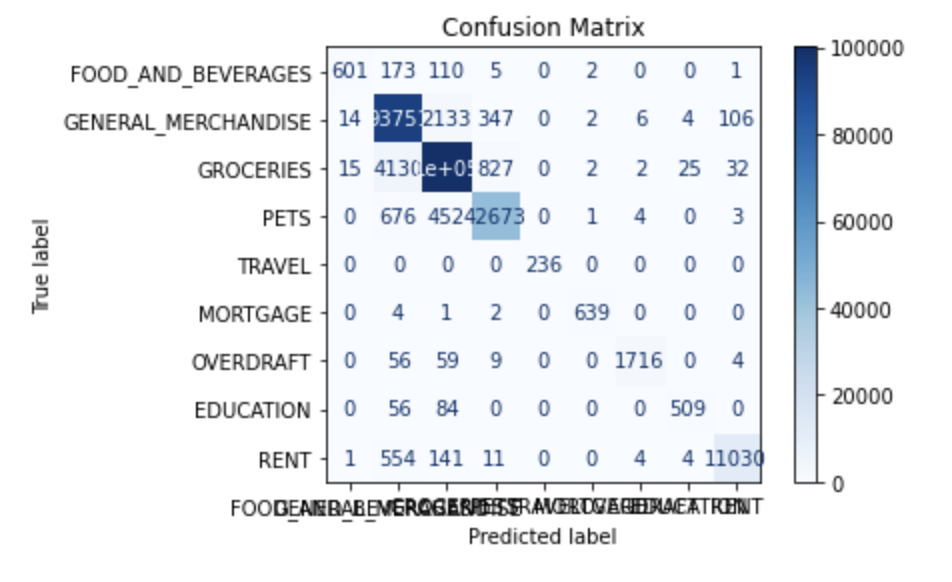
\includegraphics[width=0.8\textwidth]{figure/log_reg_confusion.png}
    \caption{Confusion Matrix for the Logistic Regression Model with TF-IDF Vectorization. The matrix shows true versus predicted labels.}
    \label{fig:confusion_matrix_logreg}
\end{figure}

\subsection{Random Forest}

Although the Random Forest model with TF-IDF vectorization was a more complex classifier, its performance did not surpass the Logistic Regression model's performance. We used the same evaluation metrics for the Random Forest model (overall accuracy, ROC-AUC scores, per-category accuracy, and the confusion matrix).

The Random Forest model achieved an overall accuracy of 84.28\% on the test set.

\subsubsection{ROC-AUC Scores and Per-Category Accuracy}
The ROC-AUC scores for each category are shown in Table \ref{table:roc_auc_rf}. These scores show that the Random Forest model had high discriminatory power in categories like \texttt{FOOD\_AND\_BEVERAGES} and \texttt{MORTGAGE}, but lower power in others, such as \texttt{EDUCATION} and \texttt{OVERDRAFT}.

\begin{table}[h]
    \centering
    \begin{tabular}{ll}
        \hline
        \textbf{Category} & \textbf{ROC-AUC Score} \\
        \hline
        GENERAL\_MERCHANDISE & 0.6648 \\
        OVERDRAFT & 0.1965 \\
        EDUCATION & 0.1667 \\
        TRAVEL & 0.4826 \\
        RENT & 0.4506 \\
        MORTGAGE & 0.7607 \\
        PETS & 0.3297 \\
        FOOD\_AND\_BEVERAGES & 0.8250 \\
        GROCERIES & 0.7506 \\
        \hline
    \end{tabular}
    \caption{ROC-AUC Scores for Each Transaction Category in Random Forest Model}
    \label{table:roc_auc_rf}
\end{table}

Table \ref{table:category_accuracy_rf} shows the per-category accuracy of the Random Forest model. Categories such as \texttt{OVERDRAFT}, \texttt{MORTGAGE}, and \texttt{RENT} achieved near-perfect accuracy, whereas categories like \texttt{FOOD\_AND\_BEVERAGES} and \texttt{GENERAL\_MERCHANDISE} had lower accuracy.

\begin{table}[h]
    \centering
    \begin{tabular}{ll}
        \hline
        \textbf{Category} & \textbf{Accuracy} \\
        \hline
        GENERAL\_MERCHANDISE & 0.8991 \\
        OVERDRAFT & 0.9998 \\
        EDUCATION & 0.9967 \\
        TRAVEL & 0.9838 \\
        RENT & 0.9984 \\
        MORTGAGE & 0.9993 \\
        PETS & 0.9960 \\
        FOOD\_AND\_BEVERAGES & 0.8476 \\
        GROCERIES & 0.9649 \\
        \hline
    \end{tabular}
    \caption{Per-Category Accuracy for Random Forest Model}
    \label{table:category_accuracy_rf}
\end{table}

\subsubsection{Confusion Matrix}
The confusion matrix for the Random Forest model (Figure \ref{fig:confusion_matrix_rf}) provides insights into its classification performance. Misclassifications are more prevalent in categories like \texttt{FOOD\_AND\_BEVERAGES} and \texttt{GENERAL\_MERCHANDISE}. This pattern suggests that the Random Forest model struggled to distinguish some categories with high similarity in text patterns.

\begin{figure}[H]
    \centering
    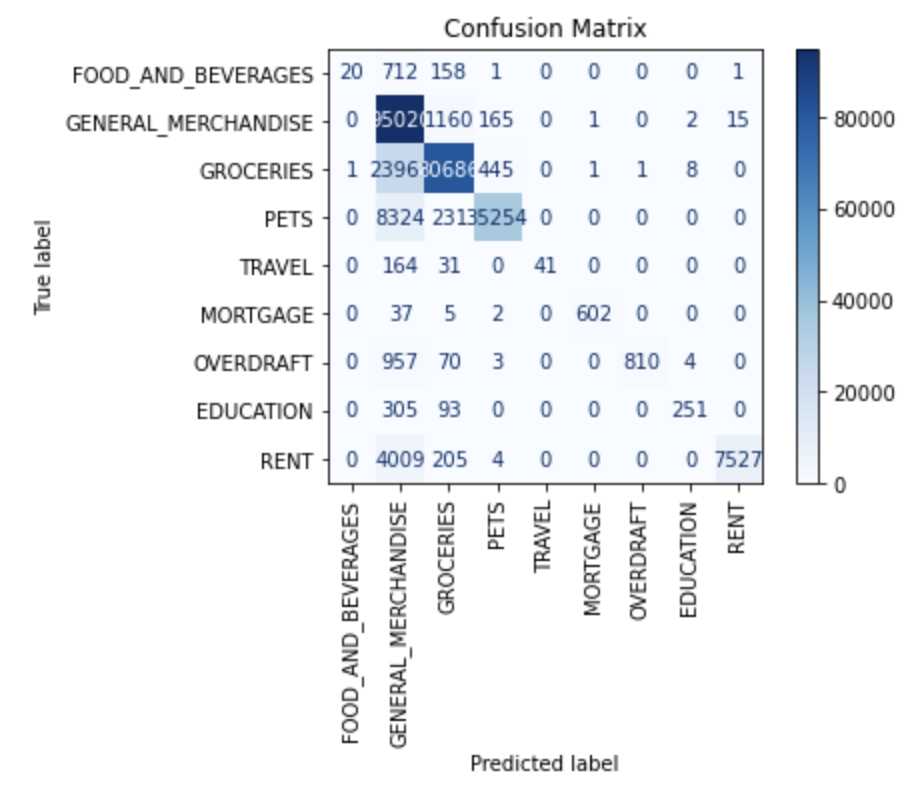
\includegraphics[width=0.8\textwidth]{figure/random_forest_confusion.png}
    \caption{Confusion Matrix for the Random Forest Model with TF-IDF Vectorization.}
    \label{fig:confusion_matrix_rf}
\end{figure}

\subsection{FastText Results}
The FastText model achieved exceptional performance, showcasing its ability to accurately classify transaction memos into categories. Below are the key outcomes from the evaluation:

\begin{itemize}
    \item \textbf{Accuracy:} The model achieved an overall accuracy of 98.93\%.
    \item \textbf{Macro Average:} Precision, recall, and F1-score values were consistently high, with a macro average F1-score of 98\%.
    \item \textbf{Weighted Average:} Weighted averages for precision, recall, and F1-score were all 99\%, highlighting the model's ability to handle class imbalances effectively.
\end{itemize}

\begin{table}[H]
    \centering
    \begin{tabular}{lcccc}
        \hline
        \textbf{Category} & \textbf{Precision} & \textbf{Recall} & \textbf{F1-Score} & \textbf{Support} \\
        \hline
        GENERAL\_MERCHANDISE & 0.98 & 0.94 & 0.96 & 892 \\
        TRAVEL               & 0.98 & 0.99 & 0.99 & 96,363 \\
        PETS                 & 0.99 & 0.99 & 0.99 & 105,107 \\
        GROCERIES            & 0.99 & 0.99 & 0.99 & 43,809 \\
        FOOD\_AND\_BEVERAGES & 1.00 & 1.00 & 1.00 & 236 \\
        EDUCATION            & 1.00 & 0.99 & 1.00 & 646 \\
        RENT                 & 0.99 & 0.99 & 0.99 & 1,844 \\
        OVERDRAFT            & 0.99 & 0.98 & 0.99 & 649 \\
        MORTGAGE             & 0.99 & 0.99 & 0.99 & 11,745 \\
        \hline
        \textbf{Overall Accuracy:} & \multicolumn{4}{c}{0.989} \\
        \hline
    \end{tabular}
    \caption{Classification Report for FastText Model}
    \label{tab:fasttext_classification_report}
\end{table}

\begin{figure}[H]
    \centering
    \includegraphics[width=0.8\textwidth]{path_to_image/confusion_matrix_fasttext.png}
    \caption{Confusion Matrix for FastText Model. Most predictions align with true categories, with minimal misclassifications.}
    \label{fig:confusion_matrix_fasttext}
\end{figure}

These results demonstrate that FastText is an effective and efficient model for classifying transaction memos. With its fast training time and high accuracy, it provides a reliable baseline for further development.

\subsection{LLM Performance}
The Transformer model was evaluated on a total of 9 transaction categories. After one epoch, it achieved a training loss of 0.1361 and a validation loss of 0.0603. The model’s validation accuracy reached 98.56\%, indicating strong generalization across categories. Evaluation on the validation set took approximately 2 minutes and 43 seconds to complete.

Although the Transformer model achieved high accuracy (98.56\%) in categorizing transaction memos, it also exhibited higher latency compared to simpler models, requiring longer processing times for both training and evaluation.

\section{Discussion}
\subsection{Interpretation of Results}

The Logistic Regression model achieved high accuracy (96.15\%) and strong ROC-AUC scores across most transaction categories, indicating that Logistic Regression, when combined with TF-IDF vectorization, is effective in distinguishing between categories based on term frequency patterns. This performance can largely be attributed to Logistic Regression's ability to handle a large number of features effectively, particularly with the addition of regularization (L2 penalty) using the \texttt{saga} solver.

Although the Random Forest model is more complex, it achieved a lower overall accuracy of 84.28\% and had mixed performance across categories. While it performed well in certain categories, such as \texttt{OVERDRAFT} and \texttt{MORTGAGE}, it struggled in others, such as \texttt{EDUCATION} and \texttt{GENERAL\_MERCHANDISE}. This discrepancy suggests that model complexity alone does not ensure better performance.

The Transformer model demonstrated the highest accuracy among the models at 98.56\%. However, the model’s high latency limit its practicality for real-time applications. 

\subsection{Model Comparison}
The likely reason for Random Forest’s lower performance lies in its sensitivity to high-dimensional, sparse data. Random Forest models work best with dense features and can struggle with the many zero-valued features produced by TF-IDF vectorization. In contrast, Logistic Regression’s performance demonstrates that it can handle sparse, high-dimensional data effectively due to its simple, linear structure and the use of regularization to prevent overfitting.

The results indicate that Logistic Regression outperformed Random Forest in both overall accuracy and category-specific ROC-AUC scores. Additionally, the confusion matrices for each model show that Logistic Regression made fewer misclassifications, with fewer off-diagonal elements overall compared to the Random Forest model.

The Transformer model, while achieving the highest accuracy at 98.56\%, comes with significant latency and requires more processing time for both training and prediction. This latency trade-off makes it unsuitable for real-time or high-frequency applications, and make the lower latency Logistic Regression a more practical choice.


\subsection{Potential Improvements}
For Random Forest, addressing feature sparsity by grouping similar words or applying dimensionality reduction techniques, such as Principal Component Analysis (PCA), could enhance performance. Further, fine-tuning hyperparameters for both models can further improve results. For Logistic Regression, using different regularization strengths could improve results, while for Random Forest, increasing the number of trees or using smaller maximum depths could improve performance.

For the limitations of Transformer models, testing smaller model architectures could potentially reduce latency

Given the mixed results of Random Forest, exploring other complex models , such as Support Vector Machines (SVMs), could provide further insight for this classification task.

\section{Inflows Analysis}
Understanding the various types of inflows is critical to assessing consumer financial behavior and identifying major income sources. This section categorizes inflows, defines what is considered income, and presents an analysis of the dataset to determine the major contributors to consumer inflows.

\subsection{Defining Inflows}
Inflows refer to any money credited to a consumer's account, including categories like \texttt{PAYCHECK}, \texttt{DEPOSIT}, \texttt{EXTERNAL\_TRANSFER}, \texttt{UNEMPLOYMENT\_BENEFITS}, and more. For this analysis, we established specific criteria for categorizing transactions:

\begin{itemize}
    \item \textbf{PAYCHECK}: Includes both \texttt{PAYCHECK} and \texttt{PAYCHECK\_PLACEHOLDER}. These transactions are typically recurrent and represent regular income, such as wages or salaries. They do not require strict recurrence to be considered income.
    \item \textbf{DEPOSIT}: Represents funds deposited directly into an account, such as checks or ATM deposits. These can be counted as income depending on the memo and recurrence.
    \item \textbf{EXTERNAL\_TRANSFER}: Includes transfers from external sources such as Venmo, Zelle, or PayPal. Regularity in the transaction pattern (e.g., weekly or monthly) and memo clustering were used to classify these as income or non-income.
    \item \textbf{OTHER\_BENEFITS}: Captures child support, social security, or other government benefits, which are considered income.
    \item \textbf{UNEMPLOYMENT\_BENEFITS}: Categorized as income, though not always recurrent.
    \item \textbf{INVESTMENT\_INCOME}: Includes dividends or other earnings from investments, counted as income.
    \item \textbf{INSURANCE}: Rarely classified as income, as these transactions typically represent reimbursements rather than earnings.
    \item \textbf{Non-Income Categories}: Categories such as \texttt{REFUND}, \texttt{SELF\_TRANSFER}, \texttt{LOAN}, and \texttt{SMALL\_DOLLAR\_ADVANCE} are excluded from income calculations as they do not contribute to a consumer's earnings.
\end{itemize}

A detailed categorization process was employed, combining memos, amounts, and recurrence patterns to ensure accurate classification. For instance, \texttt{EXTERNAL\_TRANSFER} transactions were evaluated based on their frequency, with clustering algorithms applied to group similar memos and identify patterns of recurrent inflows.

\subsection{Analysis of Inflows}
After categorizing the inflows, we analyzed their distribution across consumers and identified major sources of income. Figure \ref{fig:inflow_contributions} presents the average percentage contribution of each inflow category to total income, along with its standard deviation.

\begin{figure}[H]
    \centering
    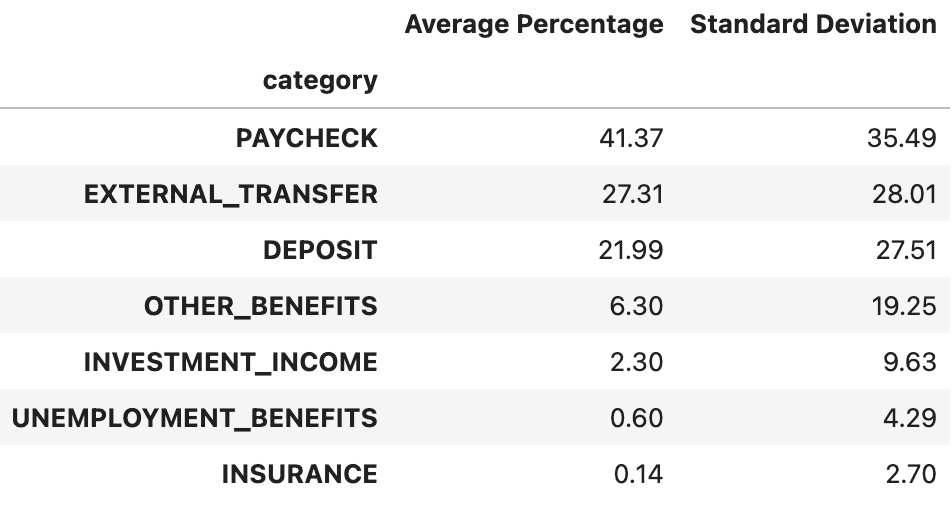
\includegraphics[width=0.8\textwidth]{figure/inflows.jpeg}
    \caption{Average Percentage Contribution of Inflows by Category with Standard Deviation. \texttt{PAYCHECK} contributes the highest percentage, followed by \texttt{EXTERNAL\_TRANSFER} and \texttt{DEPOSIT}. Categories like \texttt{UNEMPLOYMENT\_BENEFITS} and \texttt{INSURANCE} have minimal contributions.}
    \label{fig:inflow_contributions}
\end{figure}

The analysis shows that:
\begin{itemize}
    \item \textbf{\texttt{PAYCHECK}} is the largest contributor, accounting for an average of 41.37\% of total inflows, with a standard deviation of 35.49. This highlights the central role of regular wages in consumer income.
    \item \textbf{\texttt{EXTERNAL\_TRANSFER}} follows, contributing 27.31\%. Its variability (standard deviation: 28.01) suggests diverse uses, ranging from personal income (e.g., tutoring payments) to non-income transfers.
    \item \textbf{\texttt{DEPOSIT}} contributes 21.99\% on average, often representing additional sources of income like cash deposits or checks.
    \item Other categories such as \texttt{OTHER\_BENEFITS} and \texttt{INVESTMENT\_INCOME} make smaller contributions but remain important for specific subsets of consumers.
    \item Minimal contributions are observed from \texttt{UNEMPLOYMENT\_BENEFITS} (0.60\%) and \texttt{INSURANCE} (0.14\%), which are less frequent or non-recurrent sources.
\end{itemize}

This breakdown provides insight into the primary drivers of consumer inflows, particularly emphasizing the importance of recurrent sources like \texttt{PAYCHECK}. By understanding these patterns, we can develop more robust models to assess financial stability and creditworthiness.

\subsection{Statistical Insights on Inflows}
At the consumer level, we calculated several key statistics:
\begin{enumerate}
    \item \textbf{Transactions per Consumer}: The number of inflows for each consumer was computed to assess financial activity frequency.
    \item \textbf{Sum of Inflows per Consumer}: The total value of all inflows, categorized by source, was used to determine major income contributors.
\end{enumerate}

These statistics allowed us to identify the total and mean contributions of each inflow category, along with the regularity and variability of income sources. As shown in Figure \ref{fig:recurrent_vs_non_recurrent}, \texttt{PAYCHECK}, \texttt{EXTERNAL\_TRANSFER}, and \texttt{DEPOSIT} are dominant for recurrent inflows, while non-recurrent inflows show greater diversity in sources.

\begin{figure}[H]
    \centering
    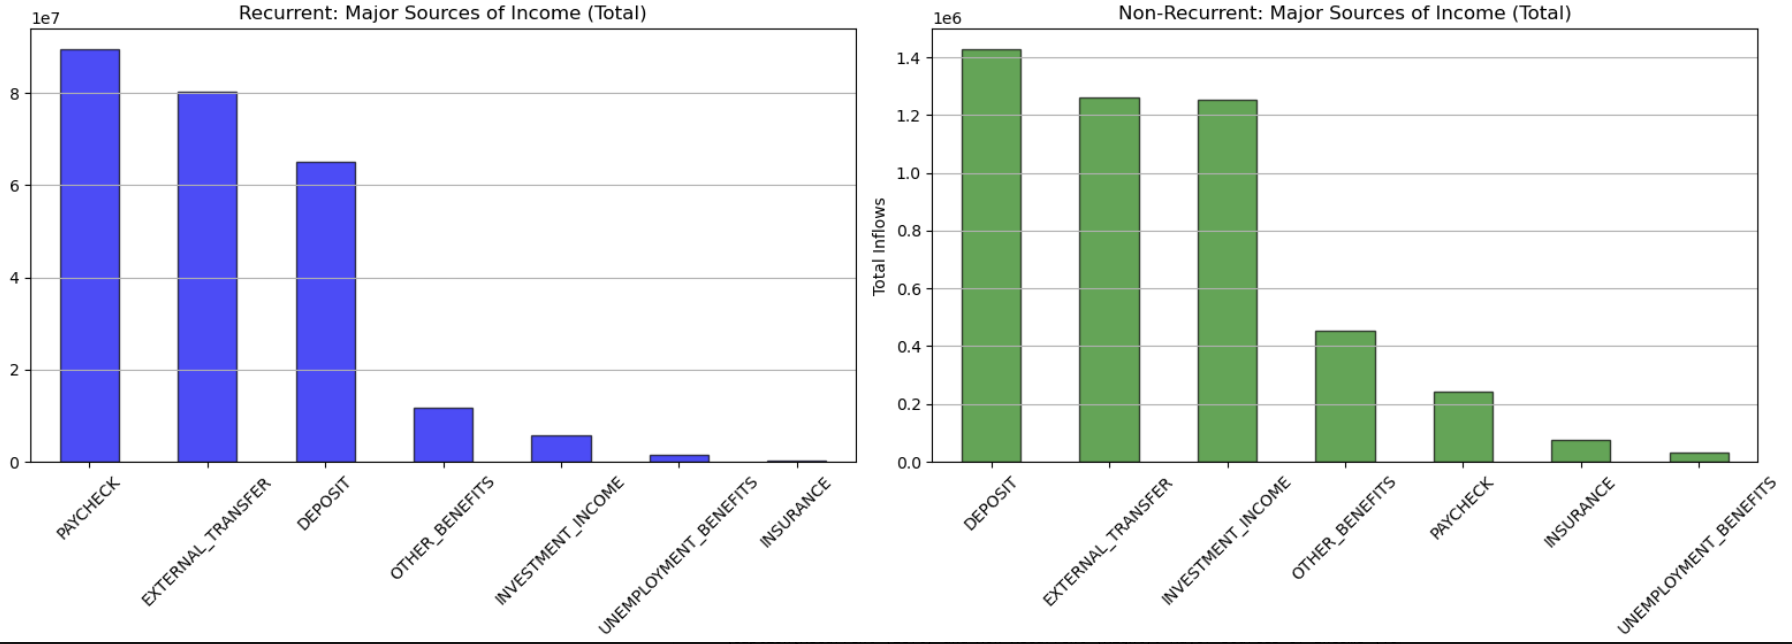
\includegraphics[width=0.8\textwidth]{figure/recurrent_vs_non_recurrent}
    \caption{Major Sources of Income for Recurrent vs. Non-Recurrent Inflows. \texttt{PAYCHECK} dominates recurrent inflows, while non-recurrent inflows have significant contributions from \texttt{DEPOSIT}, \texttt{EXTERNAL\_TRANSFER}, and \texttt{INVESTMENT\_INCOME}.}
    \label{fig:recurrent_vs_non_recurrent}
\end{figure}

This analysis highlights the critical role of recurrent income sources in consumer financial stability, while also accounting for the impact of less predictable, non-recurrent inflows.


%%%%%%%%%%%%%%%%%%%%%%%%%%%%%%%%%%%%%%%%%%%%%%%%%%%%%%%%
%%%% Literature Review and Prior Work
%%%%%%%%%%%%%%%%%%%%%%%%%%%%%%%%%%%%%%%%%%%%%%%%%%%%%%%%

\section{Literature Review}

\subsection{Attention is All You Need (2017)}

One of the key papers in machine learning, \textit{“Attention is All You Need”} by Vaswani et al. (2017), introduced the Transformer architecture along with a cohort of innovative ideas for natural language processing, becoming the foundation for modern-day language models. Specifically, the architecture addressed limitations of traditional sequence models and outdated bigram models by introducing an attention mechanism that does not rely on recurrence or convolution operations, instead focusing on weights that allow models to weigh the importance of different parts of the input sequence during processing.

This key innovation enabled Transformer models to capture long-range dependencies more effectively and efficiently compared to prior models such as RNNs and LSTMs. Additionally, Vaswani et al. demonstrated that Transformer models could achieve faster parallelism, requiring less training time.

For our application in banking transaction categorization and credit default prediction, Transformer models are particularly relevant. They offer a promising approach for future banking categorization methods due to their strong capability in self-attention, which allows precise categorization of transaction memos. This specificity enhances the richness of the data available for analysis. Furthermore, the Transformer model's ability to learn patterns in spending behavior and recognize relationships between transactions over time offers potential in detecting financial distress or increased credit risk, as it learns from sequential transaction data associated with individual consumers.

\subsection{Language Models are Unsupervised Multitask Learners (2019)}
The paper \textit{“Language Models are Unsupervised Multitask Learners”} by Radford et al. (2019) marks a shift in natural language processing by introducing GPT-2, a model that emphasizes unsupervised multitask learning. Traditionally, NLP models rely on supervised learning, where they are trained on labeled data. In contrast, GPT-2 was trained on a massive dataset without any task-specific labels, allowing it to perform multiple tasks in a \textit{zero-shot setting}, meaning it can handle tasks without additional data or fine-tuning for each one.

GPT-2’s ability to generalize across a range of tasks is primarily attributed to its use of the Transformer architecture, which employs a self-attention mechanism to capture long-range dependencies in text more effectively than previous models such as RNNs or LSTMs. The Transformer’s design also supports parallel processing, making it both faster to train and more efficient in application. For training, the authors created WebText, a massive dataset comprising data from Reddit web pages.

GPT-2’s zero-shot learning capability makes it highly adaptable for categorizing transaction memos without requiring labeled data for each specific task. By identifying patterns in transactions, GPT-2 could potentially discover trends across transaction types as well. However, despite these strengths, GPT-2 has limitations, especially in complex reasoning, which suggests room for further refinement and improvement.

\subsection{DGHNL: A new deep genetic hierarchical network of learners for prediction of credit scoring (2020)}

In financial risk management, accurate credit scoring and transaction categorization models play a crucial role in understanding borrower behavior and assessing creditworthiness. Traditional models like logistic regression offer simplicity but often fail to capture the complex, nonlinear patterns found in financial data. More advanced machine learning techniques, such as neural networks and ensemble methods, have demonstrated improved predictive accuracy by modeling these complexities. However, these approaches can be challenging to interpret, an essential factor for regulatory requirements in financial applications.
The Deep Genetic Hierarchical Network of Learners (DGHNL) offers a solution by using a combination of genetic algorithms (GAs) and hierarchical neural networks to optimize feature selection and learning in a structured, layered way. This hybrid approach is relevant to both credit scoring and transaction categorization models, as it can capture intricate patterns in bank transaction data—vital for understanding spending behaviors and identifying risky patterns. By categorizing transactions more accurately, DGHNL could support better credit assessments by providing a clearer view of a borrower’s financial habits.
DGHNL’s hierarchical architecture allows the model to focus on various data levels, potentially making it highly suitable for categorizing diverse transaction types. This structured learning enables DGHNL to balance detailed data analysis with high-level abstractions, enhancing both accuracy and interpretability. Consequently, the model not only improves risk predictions but also supports nuanced transaction categorization, helping to bridge gaps in credit scoring and financial behavior analysis.

%\bibliographystyle{IEEEtran}  % use a style that supports URLs

\clearpage

\makereference
\bibliography{reference}
\bibliographystyle{style/dsc180bibstyle}

\cite{plawiak2020dghnl}
\cite{vaswani2023attention}

\end{document}
